\newpage
\section{Theoretische Grundlagen}
\subsection{Softwarequalität}
\subsubsection{Was ist Softwarequalität?} % Zitat tüv pdf 
Wichtige Einflussfaktoren für spätere Wartungsaufwände werden bei einem großen Softwaresystem bereits zur Entwicklungszeit festgelegt. Neben einer wartungsfreundlichen und durchdachten Architektur
bestimmt vor allem die Qualität des Quellcodes darüber, ob ein System leicht verständlich, einfach durchschaubar und damit ohne große Aufwände anpassbar ist. Komplizierte Prozeduren, überlange Module, fehlende
Kommentierungen oder Verstöße gegen Coding-Standards erschweren dagegen den Durchblick und damit spätere Anpassungen durch das Wartungsteam.

% Vg Softwarequalität in PHP Projekten
Doch was verstehen wir eigentlich unter der Qualität von Software? Das bei Hewlett-Packard entwickelte FURPS ~\footcite[Vgl. S. 159]{Grady.1987} ist ein Beispiel für ein Softwarequalitätsmodell, 
das verschiedene Aspekte von Softwarequalität berücksichtigt. Die Buchstaben des Akronyms stehen für 
\begin{itemize}
	\item Functionality (Funktionalität)
	\item Usability (Gebrauchstauglichkeit)
	\item Reliability (Zuverlässigkeit)
	\item Performance (Effizienz)
	\item Supportability (Wartbarkeit)
\end{itemize}

In der Einleitung von Software-Qualität: Testen, Analysieren und Verifizieren von Software beschreibt der Autor, dass Softwarequalität facettenreich ist:

„Jedes Unternehmen, das Software entwickelt, bemüht sich, die beste Qualität auszuliefern. Man kann ein Ziel aber nur dann nachweisbar erreichen, wenn es präzise definiert ist, und das gilt für den Begriff „beste Qualität“ nicht. Softwarequalität ist facettenreich. Viele Eigenschaften einer Software ergeben gemeinsam die Software-Qualität. Nicht alle diese Eigenschaften sind gleichermaßen für den Benutzer und den Hersteller einer Software wichtig.“ ~\footcite[S 1-3]{Liggesmeyer.2009}

Die Anwender einer Applikation haben demzufolge eine andere Sicht auf die Qualität als die umsetzenden Softwareentwickler. Wir definieren diese unterschiedlichen Sichtweisen als externe beziehungsweise interne Qualität. Nigel Bevan erläutert diesen Ansatz, der in der Norm ISO/IEC 9126-1 ~\footcite[]{ISOIEC91261} spezifiziert ist, sehr ausführlich ~\footcite[]{Bevan.1999}. In den Folgenden Abschnitten findet eine genaue Betrachtung der beiden Sichtweisen statt.

\subsubsection{Interne Qualität}
Die Bedürfnisse der Entwickler beziehungsweise der Administratoren einer Anwendung machen deren interne Qualität aus. Beispielsweise ist für Softwareentwickler wichtig, dass der Code einfach zu lesen, zu verstehen, anzupassen und zu erweitern ist. Ist dies nicht der Fall, so wird es mit der Zeit immer schwieriger, die kontinuierlich gestellten und meist unvorhersehbaren Änderungswünsche des Kunden umzusetzen. Dieser weiß selber am Anfang eines Projektes nicht was die perfekte Lösung ist, da die Problemdomäne in der Regel nicht konkret greifbar für ihn ist. Irgendwann führen selbst minimale Änderungen an der Software zu unerwarteten Seiteneffekten und damit zu hohen Entwicklungskosten.

Die interne Qualität von Software ist für die Auftraggeber und Endbenutzer zunächst kaum wahrnehmbar. Für die Anwender einer Software muss diese die primär an sie gestellten funktionalen Anforderungen weitestmöglich erfüllen, und sie muss leicht und intuitiv zu bedienen sein. Ist die Anwendung bei der Abnahme dann noch „schnell genug“ ist, sind viele Auftraggeber und dessen Endanwender zufrieden.

Mangelnde oder sogar gänzlich fehlende interne Qualität wird erst auf längere Sicht spürbar. Mit der Zeit stellt man fest, dass die Bearbeitungszeit, bis scheinbar einfache bis triviale Fehler behoben sind, lang wenn nicht sogar sehr lange Zeit dauern. Erweiterungen an der Software oder Änderungen sind nur mit äußerst großem Aufwand realisierbar. In den meisten Fällen bitten die Entwickler kurz oder lang oft darum Ressourcen zu erhalten, um den Code aufzuräumen, sogenanntes refaktorieren zu betreiben. Refaktorierung wird von Fowler wie folgt beschrieben: 

\dq{}Eine Refaktorierung ist eine Änderung an der internen Struktur einer Software ohne ihr beobachtbares Verhalten zu ändern.\dq{} ~\footcite[Seite xviii]{Fowler.2000}

Oftmals wird eine solche Refaktorierung des Codes allerdings nicht (regelmäßig) durchgeführt, weil Auftraggeber oder Management den Entwicklern nicht die notwendigen Spielräume einräumen.

	Automatisierte Entwicklertests auf Modulebene sogenannte Unit-Tests, ermöglichen die unmittelbare Überprüfung, ob durch eine Änderung neue Fehler eingeführt oder bestehende Funktionalitäten unbewusst verändert wurden. Ohne diese Tests ist die Refaktorierung von Quellcode nur unter hohen Risiken möglich oder extrem hohen manuellen Testaufwänden.

Ein Ziel der Qualitätssicherung, oder genauer genommen des Projektmanagements/Qualitätsmanagements, muss daher sein, für alle am Projekt beteiligten Parteien die Kosten und den Nutzen von interner Qualität transparent und bewusst zu machen. Gelingt es, die Kosten zu quantifizieren, die durch schlechte interne Qualität langfristig entstehen, kann man darauf basierend im Rückschluss die Kostenersparnis aufzeigen, die Code von hoher interner Qualität ermöglichen würde. Das ist eine wichtige Voraussetzung dafür, das ein offizielles Budget zur Verwendung von Code-Refaktorierung berücksichtigt wird.

\subsubsection{Externe Qualität}
Der Kunde beziehungsweise der Benutzer einer Anwendung interessiert sich für diejenigen Qualitätsaspekte, die für ihn greifbar sind. Diese machen die sogenannte externe Qualität
der Anwendung aus und umfassen unter anderem:~\footcite[Vgl. Seite 5]{Bergmann.2013}
\begin{itemize}
	\item \textbf{Funktionalität} bezeichnet die Fähigkeit der Anwendung, die an sie gestellten Aufgaben den Anforderungen entsprechend zu erfüllen.
	
	\item \textbf{Gebrauchstauglichkeit} meint, dass ein Nutzer eine Anwendung effizient, effektiv und zufriedenstellend nutzen kann. Hierzu gehört auch die Barrierefreiheit.

	\item \textbf{Reaktionsfreudigkeit} bedeutet, dass die Antwortzeiten einer Anwendung auch unter Last die Benutzer zufrieden stellen. 

	\item \textbf{Sicherheit}, gerade auch die gefühlte Sicherheit der Benutzer, ist ein weiterer wichtiger Faktor für den Erfolg einer Anwendung.

	\item \textbf{Verfügbarkeit} und \textbf{Zuverlässigkeit} sind im Umfeld von Web-Plattformen mit hohem Nutzeraufkommen wichtige Themen. Die Anwendung muss auch unter großer Last funktionstüchtig sein und selbst in ungewöhnlichen Situationen sinnvoll funktionieren.
\end{itemize}

Alle Aspekte der externen Qualität haben einen Punkt gemeinsam, sie lassen sich durch End-to-End-Tests, also Tests, die eine gesamte Anwendung testen, überprüfen und validieren.

Beispielsweise werden die Anforderungen, die der Kunde an sein Produkt stellt, in sogenannten Akzeptanztests aufgeschrieben. Mit diesen Tests lässt sich automatisch verifizieren, ob die Anwendung die vom Auftraggeber erwarteten funktionalen Anforderungen erfüllt. Zusätzlich verbessern diese Akzeptanztests die Kommunikation zwischen dem Entwickler der Software und dem Kunden der diese beauftragt hat.

% rewrite open
Für Optimierungen in Bezug auf die Reaktionsfreudigkeit ist unter anderem das Messen der Reaktions- und Antwortzeit relevant. Man benötigt Werkzeuge und Techniken, mit denen man diejenigen 
Verbesserungen finden kann, die bei minimalem Aufwand und minimalen Kosten den größten Nutzen versprechen. Sowohl Entwickler als auch Administratoren sind beim Capacity Planning 
dafür verantwortlich, diejenigen Teile der Anwendung zu identifizieren, die zukünftig möglicherweise zu Flaschenhälsen, sogenannten Botlenecks, werden können, wenn die Anwendung geändert wird 
oder das Nutzeraufkommen wächst. Diese Informationen sind unverzichtbar, um die Qualität einer Anwendung in Bezug auf Verfügbarkeit und Zuverlässigkeit dauerhaft zu sichern.


\subsubsection{Technische Schulden}
Auf Ward Cunningham geht der Begriff der „technischen Schulden“ (englisch: Technical Debt) zurück:

„Although immature code may work fine and be completely acceptable to the customer,
excess quantities will make a program unmasterable, leading to extreme specialization 
of programmers and finally an inflexible product. Shipping first time code is
like going into debt. A little debt speeds development so long as it is paid back promptly
with a rewrite. Objects make the cost of this transaction tolerable. The danger occurs
when the debt is not repaid. Every minute spent on not-quite-right code counts as interest
on that debt. Entire engineering organizations can be brought to a stand-still 
under the debt load of an unconsolidated implementation, object-oriented or otherwise.“ ~\footcite[Vgl.]{website:ward:cunningham} % @todo check format

Cunningham vergleicht schlechten Quellcode mit einer Art von Hypothek, für das natürlich auch Zinsen fällig werden. Es kann durchaus sinnvoll oder gar notwendig sein, eine Hypothek aufzunehmen, wenn dadurch
das Produkt schneller vermarktungsfähig ist. Findet aber keine Tilgung der Hypothek statt, durch die Refaktorierung der Codebasis und somit eine Steigerung der interne Qualität, dann entstehen
langfristig erhebliche Kosten für die anfallenden Zinszahlungen. Wenn sich mit der Zeit die Schulden anhäufen, dann nehmen die dafür Notwendigen Zinszahlungen einem mehr und mehr den Spielraum, bis
man schließlich Konkurs anmelden muss. Auf die Software-Entwicklung übertragen bedeutet dies, dass man eine Anwendung als unwartbar bezeichnet. Die Kosten für jede noch so kleine Änderung sind so hoch gestiegen, dass es unwirtschaftlich ist, den Code weiter zu warten geschweige weiterzuentwickeln.

Mangelnde interne Qualität von Software wird besonders of dann zu einem Problem, wenn die zu entwickelnde Software an externe Agenturen/Dienstleister ausgelagert wird und der Auftraggeber primär an niedrigen Kosten und einer kurzen Time-to-Market gelegen ist. Da die Qualitätssicherung und insbesondere das Schreiben von Unit-Tests die Kosten im Projekt zunächst erhöhen, ohne dass den Kosten einen unmittelbaren und messbaren Nutzen gegenübersteht. Dadurch hat der beauftragte Dienstleister in den meisten Fällen kaum Freiräume, geschweige denn eine Motivation, um qualitativ hochwertigen Quellcode zu produzieren. Mittel- und Langfristig macht sich der Schaden für dem Auftraggeber in Form von deutlich höheren Wartungskosten bemerkbar.

Es ist daher für jedes Software-Projekt und insbesondere beim Outsourcing besonders
wichtig, dass nicht nur die zu erfüllenden Kriterien bezüglich der externen Qualität festgelegt
werden, sondern vom Auftraggeber auch ein sinnvolles Maß an interner Qualität eingefordert wird. Selbstverständlich muss der Auftraggeber dazu dem Dienstleister im Projekt auch einen gewissen finanziellen und zeitlichen Spielraum zugestehen.

Die Betriebs- und Wartungskosten für Software sind meisten zu niedrig kalkuliert da diese unterschätzt werden. Eine Realisierung eines mittelgroßes Software-Projekt dauert vielleicht ein oder zwei Jahre, die resultierende Anwendung ist aber in der Regel für Jahrzehnte in Betrieb. Jedenfalls meistens deutlich länger als bei der Planung ursprünglich gedacht.
Der größte Kostenblock für Anwendungen mit langer Nutzungsdauer sind meist der Betrieb und die Wartung. Dies gilt besonders für Anwendungen, die häufigen Änderungen unterliegen. Gerade für Webanwendungen
sind häufige Anpassungen typisch.

Andere Anwendungen die zum Beispiel für Großrechner im Finanzsektor oder hochverfügbare Telefonvermittlungen ihren Einsatz finden, müssen dagegen nur selten verändert werden. Während hier eine Änderung pro Quartal schon einen kurzen Änderungsintervall darstellt, sind für viele Webanwendungen mehrere Releases pro Monat oder sogar Wöchentlich schon längst die Regel.

Ron Jeffries ermahnt Softwareentwickler, nicht an der internen Qualität zu sparen, um die Entwicklung schneller voran zu bringen:
„If slacking on quality makes us go faster, it is clear evidence that there is room to improve our ability to deliver quality rapidly.“ ~\footcite[Vgl.]{website:jeffries.2010}

Es liegt auf der Hand, dass der Wert von interner Qualität mit zunehmender Änderungshäufigkeit von Anwendungen deutlich zunimmt. Im Artikel \dq{}The ROI of Systems Engineering: Some Quantitative Results for
Software-Intensive Systems\dq{} beschreiben die Autoren, dass die Kosten für das Beheben eines Fehlers in der Code-Phase zehnmal, in der Operations-Phase sogar mehr als hundertmal höher sind als in der Requirements-Phase. 
Dies zeigt eindeutig das es aus rein betriebswirtschaftlichen Gründen absolut widersprüchlich ist, die Kosten in einem Software-Projekt in die Zukunft zu verlagern, da die Notwendigkeit von einer guten internen Qualität 
mit Dauer des Projektes exponentiell steigt. In der Abbildung \ref{relative_kosten_von_fehlerbehebungen} ist die Kostenstruktur noch einmal visualisiert.

\begin{figure}[H]
	\begin{center}
		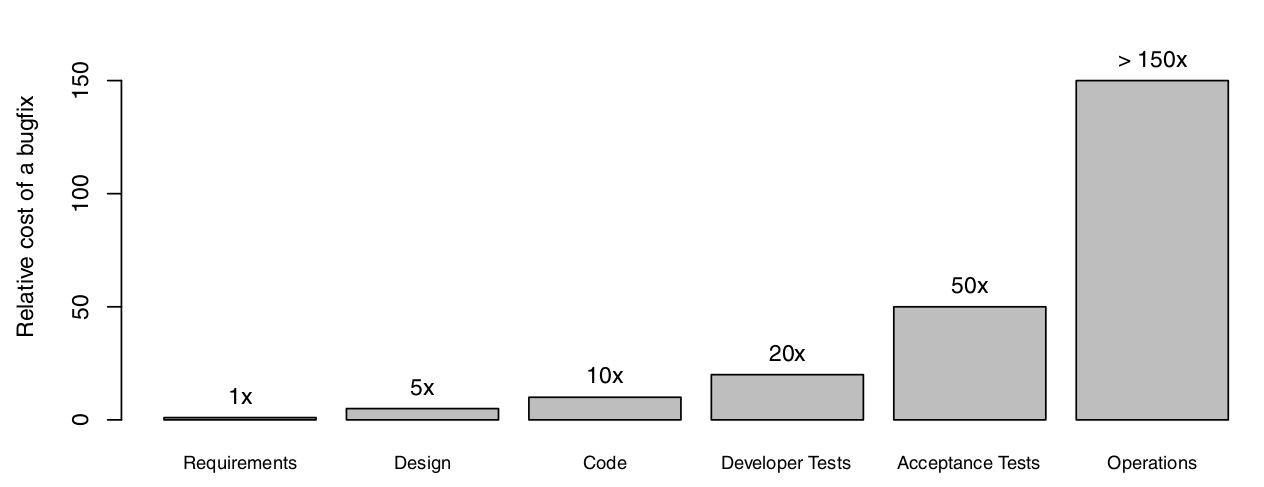
\includegraphics[width=0.9\textwidth]{relative_kosten_von_fehlerbehebungen}
		\caption{Relative Kosten von Fehlerbehebungen}
		\label{relative_kosten_von_fehlerbehebungen}
	\end{center}
\end{figure}


\subsubsection{Konstruktive Qualitätssicherung} % todo umschreiben und zitieren
Die Capability Maturity Model Integration (CMMI) und die Software Process Improvement and Capability Determination (SPICE) [ISO/IEC 15504] sowie [ISO/IEC 12207] fassen den Begriff der Qualitätssicherung enger, als er oft verwendet wird, denn das Testen wird nicht eingeschlossen [Foegen 2007]. Die Maßnahmen von CMMI und SPICE für die Aufbau- und Ablauforganisation sind jedoch die Voraussetzung für den Erfolg von analytischen Maßnahmen wie Test und Review der fertigen Software sowie konstruktiven Maßnahmen der Qualitätssicherung. [Schneider 2007] definiert konstruktive
Qualitätssicherung als Maßnahmen, die bereits bei der Konstruktion von Software auf die
Verbesserung ausgewählter Qualitätsaspekte abzielen und nicht erst nachträglich durch
Prüfung und Korrektur.

Die Erkenntnis, dass das Vermeiden von Fehlern besser ist als das nachträgliche Finden
und Beheben von Fehlern, ist nicht neu. Schon in [Dijkstra 1972] können wir lesen:

„Those who want really reliable software will discover that they must find means of
avoiding the majority of bugs to start with, and as a result the programming process
will become cheaper. If you want more effective programmers, you will discover that
they should not waste their time debugging – they should not introduce bugs to start
with.“

Ein Ansatz, der das Schreiben von fehlerhafter Software verhindern soll, ist die Test-First-
Programmierung. Sie gehört zu den technisch geprägten Praktiken, die als Bestandteil moderner 
Software-Entwicklungsprozesse zur konstruktiven Qualitätssicherung beitragen.
Der Testcode wird hierbei vor dem getesteten Code, dem sogenannten Produktionscode,
geschrieben. Die hierauf aufbauende testgetriebene Entwicklung (englisch: Test-Driven
Development) führt im Idealfall dazu, dass . . .
\begin{itemize}
	\item es keinen Produktionscode gibt, der nicht durch einen Test motiviert ist. Dies reduziert das Risiko, Produktionscode zu schreiben, der nicht benötigt wird.

	\item  es keinen Produktionscode gibt, der nicht durch mindestens einen Test abgedeckt (Code-Coverage) ist, und damit Änderungen am Produktionscode nicht zu unbemerkten Seiteneffekten führen können.

	\item testbarer Produktionscode, und damit sauberer Code (siehe nächster Abschnitt), geschrieben wird.

	\item die „Schmerzen“, die bestehender schlechter Code verursacht, verstärkt werden, da dieser nicht oder nur mit unverhältnismäßig hohem Aufwand getestet werden kann. Dies motiviert dazu, bestehenden schlechten Code durch Refaktorierung konsequent zu verbessern.
\end{itemize}

Studien wie z.B. \dq{}Software Architecture Improvement through Test-Driven Development\dq{} zeigen, dass die testgetriebene 
Entwicklung zu signifikanten Verbesserungen der Produktivität der Entwickler sowie der Softwarequalität führen kann. 
Die Anpassung zwischen konstruktiver Qualitätssicherung und normaler Softwareentwicklung ist fließend. Beispielsweise wird die Anpassbarkeit 
der Software durch den Einsatz von objektorientierter Programmierung und die Verwendung von 
Entwurfsmustern verbessert. Das entwickeln von sauberem Code (siehe nächster Abschnitt) sowie die Verwendung 
von architekturellen Mustern wie Schichtenarchitektur, serviceorientierte Architektur oder Domain-Driven Design 
führen, sofern sie richtig umgesetzt werden, zu deutlichen Verbesserungen in Bezug auf Testbarkeit, Wartbarkeit 
und Wiederverwendbarkeit der einzelnen Komponenten der Software. ~\footcite[Vgl.]{Janzen.2006}

\subsection{Clean Code}
\subsubsection{Was ist Clean Code?}
Die Frage Was ist clean Code? lässt Robert C. Martin in seinem Buch Clean Code
[Martin 2008] unter anderem Dave Thomas beantworten:

„Sauberer Code kann von anderen Entwicklern gelesen und verbessert werden. Er verfügt
über Unit- und Acceptance-Tests. Er enthält bedeutungsvolle Namen. Er stellt zur
Lösung einer Aufgabe nicht mehrere, sondern eine Lösung zur Verfügung. Er enthält
minimale Abhängigkeiten, die ausdrücklich definiert sind, und stellt ein klares und
minimales API zur Verfügung.“ ~\footcite[Vgl.]{Martin.2008}

Steve Freeman und Nat Pryce führen den Gedanken in ~\footcite[Vgl.]{Freeman.2009} mit der Aussage
fort, dass Code, der einfach zu testen ist, gut sein muss:

„For a class to be easy to unit-test, the class must have explicit dependencies that can
easily be substituted and clear responsibilities that can easily be invoked and verified.
In software-engineering terms, that means that the code must be loosely coupled and
highly cohesive – in other words, well-designed.“

In den Folgenden Abschnitten wollen wir diese Punkte genauer betrachten.

\subsubsection{Explizite und minimale Abhängigkeiten} % todo rewrite wenn möglich
Die Abhängigkeiten einer zu testenden Methode müssen klar und explizit in der API definiert sein. Das bedeutet, dass benötigte Objekte entweder an den Konstruktor der entsprechenden Klasse oder an die Methode selbst übergeben werden müssen (Dependency Injection). Die benötigten Objekte sollen nicht im Rumpf der Methode erzeugt werden, da die Abhängigkeiten sonst nicht gekapselt sind und daher nicht gegen Stub- oder Mock-Objekte ausgetauscht werden können. Je weniger Abhängigkeiten eine Methode hat, desto einfacher gestaltet sich das Schreiben ihrer Tests.

\subsubsection{Klare Verantwortlichkeiten}
Das Single Responsibility Principle (SRP) verlangt, dass eine Klasse nur für eine
fest definierte Aufgabe da ist. Sie sollte zusätzlich nur Methoden beinhalten, die direkt
zur Erfüllung dieser Aufgabe beitragen. Es sollte nie mehr als einen validen Grund geben, diese Klasse zu ändern. ~\footcite[Vgl.]{Martin.2002}

Durch dieses Prinzip ist die Verantwortlichkeit einer Klasse klar definiert und zusätzlich lassen sich ihre Methoden einfach
aufrufen und über ihre Rückgabewerte verifizieren. Somit sind alle Vorbrausetzungen für das Schreiben der entsprechenden 
Unit-Tests vorhanden und die Umsetzung dessen ist trivial.

\subsubsection{Keine Duplikation}
Eine Klasse, die versucht, zu viel zu tun, und keine klare Verantwortlichkeit hat, ist eine
hervorragende Brutstätte für duplizierten Code, Chaos und Tod ~\footcite{Fowler.2000}[Vgl.]. Duplizierter
Code erschwert die Wartung der Software, da die Konsistenz zwischen den einzelnen Duplikaten gewährleistet 
sein muss. Ein Fehler der von deinem ggf. neu an dem Projekt beteiligten Softwareentwickler behoben wird, 
ist nicht zwangsläufig an allen duplizierten Stellen behoben. Dies führt zu schwierigen Fehlersuchen und 
erhöht die Anfälligkeit der Software für Seiteneffekte. 

\subsubsection{Kurze Methoden mit wenigen Ausführungszweigen}
Eine Methode ist umso schwerer zu verstehen, je länger sie ist. Eine kurze Methode lässt
sich nicht nur einfacher verstehen und wiederverwenden, sondern ist auch einfacher zu
testen. Je weniger Ausführungspfade eine Methode hat, desto weniger Tests werden benötigt. ~\footcite[Vgl. Seite 9]{Bergmann.2013}

\subsection{Software-Metriken}\label{software-metriken}
Für das Messen der internen Qualität gibt es verschiedene Software-Metriken. Sie sind eine Grundlage für das Quantifizieren der Kosten, die durch schlechte interne Qualität langfristig entstehen.

Testbarkeit ist ein wichtiges Kriterium für die Wartbarkeit im Softwarequalitätsmodell von ISO/IEC 9126-1~\footcite{ISOIEC91261}[Vgl.]. Es in der Literatur mehrere Beispiele für Ansätze zur Quantifizierung von Testbarkeit basierend auf objektorientierten Software-Metriken. ~\footcite[Vgl. Seite 136-145]{Bruntink.2004} ~\footcite[Vgl. Seite 1 - 6]{Khan.2009}

Einen weiteren guten Überblick über objektorientierte Software-Metriken ist im Buch von gibt beispielsweise im Buch \dq{}Object-Oriented Metrics in Practice: Using Software Metrics to Characterize, Evaluate, and Improve the Design of Object-Oriented Systems\dq{} von Michele Lanza und Radu Marinescu. ~\footcite[Vgl.]{Lanza.2006}

Man darf jedoch niemals vergessen, dass Metriken lediglich Indikatoren für Qualitätsprobleme sind. Metriken sollten immer als Hinweise auf bestimmte Stellen im Code verstanden werden,
die man sich als Mensch ansehen sollte, um jeweils selbst zu beurteilen, ob und im welchem Maße der Code tatsächlich problematisch ist.

Im Folgenden betrachten wir einige Software-Metriken, die für die Testbarkeit besonders relevant sind.

\begin{itemize} %todo rewrite
	\item \textbf{Zyklomatische Komplexität und NPath-Komplexität}
	Die zyklomatische Komplexität (englisch: Cyclomatic Complexity) ist die Anzahl der möglichen Entscheidungspfade 
	innerhalb eines Programms beziehungsweise innerhalb einer Programmeinheit, normalerweise einer Methode oder Klasse. ~\footcite[Vgl. Seite 1-3]{McCabe.1976}
	Sie wird durch Zählen der Kontrollstrukturen und booleschen Operatoren innerhalb der Programmeinheit 
	berechnet und sagt etwas über die strukturelle Schwierigkeit einer Programmeinheit aus. McCabe geht davon aus, 
	dass die einfache Abfolge von sequenziellen Befehlen einfacher zu verstehen ist als eine Verzweigung im Programmfluss.

	Eine hohe zyklomatische Komplexität ist ein Indikator dafür, dass eine Programmeinheit
	anfällig für Fehler und schwer zu testen ist. Je mehr Ausführungspfade eine Programmeinheit hat, 
	desto mehr Tests werden benötigt. Die NPath-Komplexität ~\footcite[Vgl. Seite 188-200]{Nejmeh.1988} zählt die azyklischen Ausführungspfade. 
	Um die Anzahl der Ausführungspfade endlich zu halten und redundante Informationen auszuschließen, berücksichtigt die NPath-Komplexität
	nicht jeden möglichen Schleifendurchlauf.
	
	\item \textbf{Change Risk Anti-Patterns (CRAP) Index}
	Der Change Risk Anti-Patterns (CRAP) Index, ursprünglich als Change Risk Analysis and Predictions Index bekannt, 
	sagt nicht direkt etwas über die Testbarkeit aus. Er soll an dieser Stelle aber nicht unerwähnt bleiben, da er sich 
	neben der Cyclomatic Complexity auch aus der durch die Tests erreichten Code-Coverage berechnet.
	
	Code, der nicht zu komplex ist und über eine ausreichende Testabdeckung verfügt, weist
	einen niedrigen CRAP-Wert auf. Das Risiko, dass Änderungen an diesem Code zu unerwarteten 
	Seiteneffekten führen, ist geringer als bei Code, der einen hohen CRAP-Wert aufweist.
	Letzteres ist für komplexen Code mit wenigen oder sogar gar keinen Tests der Fall.
	
	Der CRAP-Wert kann entweder durch das Schreiben von Tests oder durch eine geeignete Refaktorierung 
	gesenkt werden. Beispielsweise helfen die Refaktorierungen Methode extrahieren und Bedingten Ausdruck 
	durch Polymorphismus ersetzen dabei, eine Methode zu verkürzen und die Anzahl der möglichen 
	Entscheidungspfade – und damit die zyklomatische Komplexität – zu verringern.
	
	\item \textbf{Kohäsion und Kopplung}
	
	Ein System mit starker Kohäsion besteht aus Komponenten, die nur für genau eine spezifizierte Aufgabe 
	zuständig sind. Eine lose Kopplung ist dann erreicht, wenn Klassen voneinander weitgehend unabhängig 
	sind und nur durch wohldefinierte Schnittstellen miteinander kommunizieren [Yourdon 1979].
	
	Das Gesetz von Demeter ~\footcite[Vgl. Seite 67-78]{Lieberherr.1989}verlangt, dass eine Methode eines Objekts nur Methoden desselben 
	Objekts sowie von an die Methode per Parameter übergebenen und 	in der Methode erzeugten Objekten aufrufen darf. 
	Die Einhaltung dieses Gesetzes führt zu loser Kopplung. Für die Testbarkeit ist es wichtig, auf das Erzeugen von Objekten im
	Rumpf einer Methode zu verzichten, um so alle ihre Abhängigkeiten gegen Stub- oder
	Mock-Objekte austauschen zu können. Es gibt empirische Belege, dass Verstöße gegen
	das Gesetz von Demeter Indikatoren für die erhöhte Fehleranfälligkeit einer Software sind.[Guo 2011]
	
\end{itemize}

\subsection{Testen von Software}\label{arten-von-tests} 
\subsubsection{Einführung} %todo rewrite
In der klassischen, nicht-iterativen Software-Entwicklung sind Programmierung sowie
Integrations- und Systemtests zwei getrennte Phasen im Projekt, die oft von unterschiedlichen
Teams durchgeführt werden. Es ist durchaus sinnvoll, wenn die Entwickler nicht
ihre eigene Arbeit testen. Ein unabhängiger Tester hat eine ganz andere Sichtweise auf
die zu testende Anwendung, da er die Implementierung nicht kennt. Er kann also nur
die Bedienoberfläche (oder Schnittstelle) einer Anwendung testen. Dabei bedient er die
Anwendung ganz anders als ein Entwickler, der beim Test noch den Code vor Augen hat
und daher intuitiv vorwiegend die Funktionalität überprüft, von der er eigentlich weiß,
dass sie funktioniert. Ein unabhängiger Tester – bewährt haben sich übrigens auch Tests
durch Personen, die zum ersten Mal mit der zu testenden Anwendung arbeiten – entwickelt
im Idealfall ausreichend destruktive Kreativität, um die Arbeit des Entwicklers auf
eine harte Probe zu stellen und die Anwendung etwa mit wirklich unsinnigen Eingaben,
abgebrochenen Aktionen oder etwa manipulierten URLs herauszufordern.

Tests, die ohne Kenntnis der Implementierung durchgeführt werden, nennt man Black-
Box-Tests. Tests, die anhand des Quellcodes der zu testenden Anwendung entwickelt wer-
den, nennt man dagegen White-Box-Tests.

Auf den ersten Blick scheint das Testen von Webanwendungen besonders einfach zu sein.
Das zu testende Programm erhält einen HTTP-Request, also einen String, vom Browser
und erzeugt einen HTML-String, der an den Browser zurückgesendet und dort dargestellt
wird. Natürlich können auch andere Ausgabeformate wie JSON oder XML erzeugt werden,
aber auch diese sind nur Zeichenketten. Ein Test der Webanwendung muss überprüfen, ob
das Programm für eine bestimmte Eingabe-Zeichenkette die korrekte erwartete Ausgabe-
Zeichenkette erzeugt.

Während es in der Tat relativ einfach ist, die Korrektheit der Ausgabe für eine Eingabe zu
prüfen, macht es bereits die unüberschaubar große Anzahl von möglichen Eingaben unmöglich 
zu überprüfen, ob das Programm für alle möglichen Eingaben eine korrekte Ausgabe erzeugt. 
Ein Programm erhält (leider) nicht nur sinnvolle Eingaben, deshalb kann man sich nicht
einfach darauf zurückziehen, nur einige wenige sinnvolle Eingaben zu testen. In einer 
URL sind 73 verschiedene Zeichen (die alphanumerischen Zeichen in Klein-und Großschrift 
sowie einige Sonderzeichen) erlaubt, alle weiteren Zeichen müssen URL-kodiert werden. 
Würde man versuchen, alle URLs bis zu einer Länge von 20 Zeichen aufzuzählen 
(es gibt mehrere Sextillionen solcher URLs), und könnte 
pro Sekunde eine Million URLs aufzählen, dann bräuchte man dafür rund $10^{23}$ Jahre. Das bedeutet 
in der Praxis, dass man diese Aufgabe niemals fertigstellen wird, da die Sonne in voraussichtlich $10^{9}$
Jahren zu einer Supernova wird und dabei die Erde vernichtet.

Durch Bildung von Äquivalenzklassen kann man die Anzahl der zu testenden Eingaben
erheblich reduzieren. Unter einer Äquivalenzklasse versteht man eine Menge von Eingaben,
für die der Programmablauf identisch ist, auch wenn mit anderen Variablen gerechnet wird. 
Nehmen wir an, Sie wollen ein Programm testen, das eine gegebene ganze Zahl inkrementiert. 
Es ist egal, ob dieses Programm eine Inkrement-Operation oder eine Addition verwendet 
(oder ganz anderes implementiert ist). Wenn wir davon ausgehen, dass PHP korrekt funktioniert, 
dann reicht es, eine einzige repräsentative Eingabe zu testen. Liefert das Programm für 
diese Eingabe ein richtiges Ergebnis, dann können wir davon ausgehen, dass es korrekt funktioniert, 
ohne dass wir es für alle ganzen Zahlen aufgerufen haben.

Besondere Beachtung verdienen Grenzwerte und unzulässige Eingaben. Diese bilden neben
den „normalen“ Eingaben weitere Äquivalenzklassen, die ebenfalls jeweils einen Test
erfordern. Was geschieht beispielsweise, wenn wir die höchste darstellbare Integer-Zahl 
inkrementieren? Und was geschieht, wenn wir versuchen, nichtnumerische Werte, beispielsweise
eine Zeichenkette, zu inkrementieren?

In der Praxis ist es nicht immer ganz einfach, die Äquivalenzklassen zu identifizieren 
beziehungsweise mit repräsentativen Eingaben zu testen. Als Faustregel gilt, dass man immer
zuerst den Erfolgsfall, den sogenannten \textit{Happy Path}, testen sollte. Danach widmet man
sich Grenzwerten, also beispielsweise dem höchsten zulässigen Wert sowie dem höchsten
zulässigen Wert plus eins beziehungsweise dem niedrigsten Wert und seinem Vorgänger.
Nun kann man unsinnige Eingaben testen, etwa NULL-Werte oder falsche Datentypen.

Für Black-Box-Tests ist das Identifizieren von Äquivalenzklassen schwieriger als für White-Box-Tests,
bei denen man sich an den Fallunterscheidungen beziehungsweise den verschiedenen Ausführungspfaden orientieren kann.

Da HTTP ein zustandsloses Protokoll ist, gibt es per Definition keinerlei Abhängigkeiten
zwischen zwei aufeinanderfolgenden HTTP-Requests. Das Testen einer auf HTTP basierenden 
Anwendung scheint also wiederum besonders einfach, da jeder HTTP-Request, also jede Eingabe,
nur ein einziges Mal getestet werden muss.

Wie wir aber alle wissen, wird die Zustandslosigkeit von HTTP in den meisten Webanwendungen
durch die Verwendung von Cookies und eine serverseitige Session-Verwaltung durchbrochen. 
Ohne einen Zustand könnte die Anwendung nicht zwischen einem anonymen und einem angemeldeten
Benutzer unterscheiden, beziehungsweise man müsste die Zugangsdaten mit jedem HTTP-Request erneut übertragen.

Da eine zustandsbehaftete Anwendung je nach ihrem Zustand unterschiedlich auf Eingaben reagieren kann,
reicht es noch nicht einmal mehr aus, alle möglichen Eingaben zu testen, obwohl wir schon wissen, 
dass es davon deutlich mehr gibt, als uns lieb sein kann. Um eine zustandsbehaftete Anwendung
vollständig zu testen, müssten wir das Programm auch mit allen möglichen Abfolgen von Eingaben testen.

Ein typisches Beispiel für zustandsabhängig variables Verhalten ist etwa der Versuch, auf
nicht öffentliche Inhalte zuzugreifen. Ein anonymer Besucher wird aufgefordert, sich anzumelden,
während ein angemeldeter Benutzer die entsprechenden Inhalte zu sehen bekommt, zumindest wenn er
die dazu nötigen Berechtigungen besitzt. 

Es bedarf wohl keiner weiteren Überschlagsrechnungen, um zu zeigen, dass es unmöglich 
ist, einen umfassenden Test einer Webanwendung vor dem Weltuntergang zu Ende zu bringen, 
wenn es uns noch nicht einmal annähernd gelingt, in dieser Zeit alle möglichen
Eingaben aufzuzählen.

\subsubsection{Systemtests}
\paragraph{Manuelle Tests im Browser} %todo rewrite
Einer der großen Vorteile von PHP-Anwendungen ist, dass man gerade geschriebenen Code
direkt ausführen und das Ergebnis im Browser ansehen kann. Dieses direkte Feedback
ist vermutlich einer der Hauptgründe, warum viele Entwickler PHP gegenüber einer über-
setzten Sprache wie Java bevorzugen. Was liegt also näher, als die Anwendung insgesamt
im Browser zu testen?

Heutzutage generieren PHP-Anwendungen längst nicht mehr nur statisches HTML. Mittels
JavaScript kann im Browser der DOM-Baum des HTML nahezu beliebig manipuliert wer-
den. So können jederzeit Seitenelemente geändert, hinzugefügt oder verborgen werden.
In Verbindung mit asynchron abgesetzten HTTP-Requests an den Server, auf die als 
Antwort meist XML- oder JSON-Datenstrukturen zum Browser zurückgesendet werden, lässt
sich das ansonsten nötige Neuladen der Seite vermeiden. Dank AJAX erlebt der Benutzer
heute im Web teilweise einen Bedienkomfort, wie es bis vor einigen Jahren ausschließlich
klassischen GUI-Anwendungen vorbehalten war.

Durch den Einsatz von AJAX wird allerdings auch im Browser die Zustandslosigkeit des
HTTP-Protokolls aufgehoben. Das dargestellte HTML-Dokument wird mehr und mehr zu
einer eigenen Client-Anwendung, die über AJAX-Anfragen mit dem Server kommuniziert
und ihren eigenen, technisch gesehen vom Server völlig unabhängigen Zustand hat. Der
Programmierer sieht sich plötzlich mit zusätzlichen Aufgaben konfrontiert, die zuvor in
der Webprogrammierung keine große Rolle gespielt haben, beispielsweise mit Locking-
Problemen sowie dem Umgang mit Verklemmungen (englisch: Deadlocks) und Timeouts.
Es genügt also in den meisten Fällen längst nicht mehr, das durch eine PHP-Anwendung
generierte HTML-Dokument statisch zu analysieren, um die syntaktische Korrektheit 
beziehungsweise, wenn XHTML zum Einsatz kommt, die Wohlgeformtheit zu überprüfen
und durch mehr oder minder aufwendiges Parsing sicherzustellen, dass die Seite (nur) die
gewünschten Informationen enthält.

Da heute ein zunehmender Teil der Funktionalität einer Anwendung in JavaScript implementiert 
wird, muss für einen umfassenden Test auch der JavaScript-Code ausgeführt werden. 
Man könnte dazu eine JavaScript-Engine wie Rhino, SpiderMonkey oder V8 verwenden.
Da man aber früher oder später auch die Darstellung der Seite überprüfen möchte,
führt letztlich am Test im Browser kein Weg vorbei. Wie wir wissen, hat jede 
Browser-Familie beziehungsweise jede Browser-Version ihre Eigenheiten nicht nur bezüglich der
Darstellung, sondern auch bezüglich der Ausführung von JavaScript-Code. Obwohl sich
die Situation in den letzten Jahren deutlich gebessert hat, können die kleinen Browser-
Unterschiede den Entwicklern einer Webanwendung das Leben ganz schön schwer machen.

Verhält sich eine Anwendung im Browser-Test nicht wie erwartet, ist es oft nur schwer möglich,
die tatsächliche Fehlerquelle zu lokalisieren. Ist das Problem auch in anderen Browsern 
vorhanden? Ändert sich das Verhalten eventuell mit anderen Sicherheitseinstellungen?
Ist die Ursache des Fehlers ungültiges HTML oder ein Fehler im JavaScript- oder PHP-Code?
Spielt etwa die Datenbank eine Rolle?

Es ist ein generelles Problem von Systemtests, an denen naturgemäß viele Komponenten
beteiligt sind, dass man die Ursache von Fehlern nur schwer einkreisen kann. Ein fehlgeschlagener
Test, egal ob manuell oder automatisiert durchgeführt, zeigt zwar, dass die getestete
Software nicht wie erwartet funktioniert, gibt aber keine Auskunft darüber, wo der
Fehler liegen könnte.

Im letzten Abschnitt wurde bereits ausgeführt, dass es unmöglich ist, eine Anwendung
auch nur annähernd mit allen möglichen Eingaben zu testen. Selbst wenn wir uns darauf
beschränken, alle Geschäftsvorfälle oder Geschäftsregeln mit jeweils einer repräsentativen
Eingabe zu testen, erreichen wir schnell eine nicht mehr beherrschbare Komplexität. In einem
sozialen Netzwerk muss beispielsweise jeder Freund den neuesten Blog-Eintrag eines
Benutzers kommentieren dürfen. Kommt Moderation ins Spiel, dann darf ein Kommentar
zunächst für niemanden sichtbar sein (außer vielleicht für den Moderator und den Autor
des Kommentars), muss aber nach der Freischaltung sichtbar werden. Darf der Autor
des Kommentars diesen nun löschen oder ändern? Muss eine Änderung erneut moderiert
werden?

Um Geschäftsregeln wie diese zu testen, müsste man sich abwechselnd mit mindestens
zwei verschiedenen Benutzerkonten an der Anwendung anmelden. Selbst wenn man sich
diese Mühe macht, steht man spätestens vor dem nächsten Release der Anwendung vor
der Frage, ob man nun alle Tests wiederholen möchte oder einfach riskiert, dass die 
Anwendung aufgrund von unerwünschten Nebeneffekten einer Änderung nicht mehr wie erwartet
funktioniert.

Allein das Erstellen eines Testplanes, der beschreibt, welche Geschäftsvorfälle beziehungsweise
Geschäftsregeln zu testen sind, welche Aktionen dazu notwendig und welche Ergebnisse zu
erwarten sind, ist eine langwierige Arbeit. Auf der anderen Seite dient ein Testplan
auch dazu, die funktionalen Anforderungen an die Anwendung zu dokumentieren.
Der Testplan ist damit die Basis für Akzeptanztests, mit denen der Kunde prüft, ob die 
Software die an sie gestellten Anforderungen erfüllt.

\paragraph{Automatisierte Tests}
Da das manuelle Testen einer Anwendung zeitintensiv und nervenaufreibend ist, bietet es
sich an, Tests so weit wie möglich zu automatisieren. Durch Automation wird nicht nur die
Ausführungsgeschwindigkeit erhöht, sondern auch Flüchtigkeitsfehler werden vermieden.
Abgesehen vom Stromverbrauch entstehen keine Mehrkosten, wenn man die Tests wiederholt
ausführt. Testautomation ist damit eine wichtige Voraussetzung, um Anwendungen
mit verschiedenen Betriebssystemen, Datenbanken, PHP-Versionen und -Konfigurationen
testen zu können.

Ein erster Ansatz, Tests im Browser zu automatisieren, sind die sogenannten „Capture and
Replay“-Werkzeuge. Im einfachsten Fall zeichnen diese die Mausbewegungen und Eingaben
auf und können diese später wiedergeben. Da gerade Webanwendungen mit verschiedenen
Fenstergrößen und Bildschirmauflösungen betrieben werden, sollte die Aufzeichnung nicht
auf Bildschirmpositionen abstellen, sondern besser die im Browser ausgelösten
Ereignisse auf DOM- beziehungsweise JavaScript-Ebene aufzeichnen.

Die freie Software Selenium ist ein Werkzeug, das in Form einer Firefox-Erweiterung die
Aufzeichnung und Ausführung von Browser-Tests ermöglicht. Ein in Java geschriebener
Proxy-Server ermöglicht im Zusammenspiel mit PHPUnit auch die Fernsteuerung eines
Browsers aus einem PHPUnit-Test. Somit können Browser-Tests auch im Rahmen von 
kontinuierlicher Integration ausgeführt werden.
In den Selenium-Tests kann man mit Zusicherungen auf den DOM-Baum sicherstellen,
dass die gerade dargestellte HTML-Seite bestimmten Prüfkriterien genügt. Da der Test 
direkt im Browser ausgeführt wird, wird der JavaScript-Code in der Seite ausgeführt, somit
lassen sich auch AJAX-Anwendungen mit Selenium testen.

In den Zusicherungen kann unter anderem das Vorhandensein oder der Inhalt beliebiger
HTML-Elemente geprüft werden. Der Zugriff auf die einzelnen Elemente beziehungsweise
DOM-Knoten erfolgt entweder über HTML-IDs, CSS-Selektoren, mittels JavaScript-Code
oder mit einem XPath-Ausdruck. Da die Fernsteuerung des Browsers in JavaScript, das in
die zu testende Seite injiziert wird, realisiert ist, gibt es beim Testen allerdings einige 
Einschränkungen, die auf Sicherheitsbeschränkungen zurückzuführen sind. Es ist beispielsweise
nicht möglich, einen Datei-Upload zu testen, da dazu das im Browser ausgeführte
JavaScript auf das Dateisystem des Rechners zugreifen müsste, um die hochzuladende Datei
auszuwählen. Man möchte aus naheliegenden Gründen normalerweise nicht, dass der
JavaScript-Code einer Website Zugriff auf das lokale Dateisystem hat. In manchen Browsern
lassen sich Einschränkungen in speziellen Betriebsmodi umgehen. Firefox etwa kann
man in den Chrome-Modus schalten, in dem deutlich weniger Sicherheitsbeschränkungen
für JavaScript-Code gelten.

Systemtests, die eine Anwendung durch die Benutzeroberfläche testen, sind wie alle indirekten
Tests eher fragil. Eine scheinbar harmlose Änderung am Layout der Benutzeroberfläche,
etwa weil die Werbung eines wichtigen Kunden prominent platziert werden muss,
kann schon dafür sorgen, dass Zusicherungen fehlschlagen, obwohl eigentlich nur eine
kosmetische Änderung an der Anwendung vorgenommen wurde. Es bedarf einiger Vorsicht
und einer umsichtigen Planung sowohl der Seitenstruktur als auch der Zusicherungen,
um vor zu häufig zerbrechenden Tests einigermaßen geschützt zu sein.

\paragraph{Akzeptanztests}
Systemtests sind normalerweise Black-Box-Tests, sie werden also ohne Kenntnis von Interna
der zu testenden Software erstellt und durchgeführt. Akzeptanztests sind Systemtests,
die aus der Sicht des Endbenutzers beziehungsweise des Kunden erstellt werden und prüfen,
ob eine Anwendung die Spezifikation erfüllt und die erwartete Funktionalität hat.
Zumindest bezüglich der funktionalen Aspekte sind die Akzeptanztests mit einem Werkzeug 
wie Selenium einfach automatisierbar. Akzeptanztests sind auch dann sinnvoll, wenn
Sie Software nur für die eigene Verwendung entwickeln, da Sie auf diese Weise im Sinne der
testgetriebenen Programmierung gezwungen sind, sich von vornherein Gedanken über die
Funktionalität aus Endbenutzersicht zu machen, ohne über die konkrete Implementierung
nachzudenken.

Die wichtigste Eigenschaft von Akzeptanztests ist, dass diese Abweichungen von der 
Spezifikation aufzeigen können. White-Box-Tests orientieren sich am vorhandenen Code und
man nutzt Metriken für die Codeabdeckung (englisch: Code-Coverage) wie Statement Coverage,
Line Coverage und Path Coverage, um fehlende Testfälle zu finden. Wenn eine von
der Software geforderte Funktionalität nicht realisiert ist, dann gibt es dafür allerdings
keinen zu testenden Code, also kann ein White-Box-Test nicht aufdecken, dass die Software
von der Spezifikation abweicht. Ein Black-Box-Test dagegen, der sich von vornherein nur
an der geforderten Funktionalität orientiert, kann auch auf fehlenden Code hinweisen.

\paragraph{Grenzen von Systemtests}
Gewisse nicht-funktionale Aspekte wie Layout-Defekte oder mangelnde Gebrauchstauglichkeit 
lassen sich nicht automatisiert testen. Zwar ist es denkbar, etwa beim Testen
Screenshots zu erstellen und diese automatisiert zu vergleichen. Allerdings kann bis heute
keine Maschine das menschliche Auge ersetzen, wenn es darum geht, die Harmonie eines
Entwurfes oder die subjektive Wahrnehmbarkeit eines Designelements zu beurteilen.
Gerade in Projekten, die über mehrere Monate oder gar Jahre andauern, ist es problematisch,
wenn man mit dem Testen erst dann beginnen kann, wenn die Software weitgehend
fertiggestellt ist. Wenn man die Tests automatisiert und auf manuelles Testen verzichtet, ist
es zwar kein Problem, die Tests beliebig oft zu wiederholen, während die Software wächst.
Es wird aber dennoch einige Zeit dauern, bis die ersten Tests durchgeführt werden können.
Es wäre wünschenswert, mit dem Testen schon deutlich früher im Entwicklungsprozess
beginnen zu können.

Systemtests sind relativ langsam, da sie eine komplexe Test-Umgebung benötigen und alle
Komponenten der Anwendung vom Browser über den Webserver bis zur Datenbank beteiligt sind.
Es mag kein Problem sein, vor dem Release einer neuen Software-Version einen
mehrstündigen Test durchzuführen. Immerhin sind automatisierte Tests deutlich schneller
als manuelle Tests. Will man aber den Entwicklern im Rahmen ihrer täglichen Arbeit ein
schnelles Feedback darüber geben, ob sie mit einer Änderung unerwünschte Nebeneffekte
eingeführt haben, stößt man schnell an die Grenzen von Systemtests, zumal diese nicht
einfach parallel ausgeführt werden können, da sie Abhängigkeiten von einer Datenbank,
Caches und möglicherweise Dateien im Dateisystem haben. Kommen sich dabei mehrere
Tests in die Quere, führt dies schnell zu Fehlern, die sich nicht reproduzieren lassen. Das
ist das genaue Gegenteil von dem, was Systemtests eigentlich leisten sollen.

\subsubsection{Unit-Tests}
Im Gegensatz zu End-to-End-Tests, die eine gesamte Anwendung testen, testet man mit
Unit-Tests nur einen Teil (englisch: Unit) einer Anwendung, meist nur eine einzelne Klasse,
manchmal aber auch ein Aggregatobjekt. Unit-Tests sind normalerweise White-Box-Tests,
da man sie unter Berücksichtigung des zu testenden Quelltextes schreibt.

Viele Entwickler haben das Ziel, mit Unit-Tests eine hohe Codeabdeckung zu erreichen, also
im Rahmen der Tests möglichst jede Zeile des Produktionscodes auszuführen. Mit der
PHP-Erweiterung Xdebug können beim Testen Informationen über die Line Coverage gesammelt
werden, die von PHPUnit aufbereitet und im HTML-Format visualisiert oder als
Text oder XML gespeichert werden können.

Diese zeilenbasierte Codeabdeckung berücksichtigt nicht, dass der getestete Code im
Allgemeinen mehrere Ausführungspfade hat. Die bereits vorgestellte NPath-Komplexität
ist ein Maß für die Anzahl der Ausführungspfade in einem Codeabschnitt. Sie
gibt an, wie viele Tests nötig sind, um eine vollständige Pfadabdeckung zu erreichen, also
um nicht nur jede Codezeile, sondern auch jeden Ausführungspfad mindestens einmal zu
durchlaufen.

Die zeilenbasierte Codeabdeckung allein ist also kein Nachweis für umfassende Tests, sondern
dient im Gegenteil an sich nur dazu, zu zeigen, welche Teile des Codes noch vollständig
ungetestet sind. Es gibt derzeit kein Werkzeug für PHP, mit dem sich Pfadabdeckungsstatistiken
erstellen lassen. Es gibt allerdings Bestrebungen Xdebug und PHPUnit in diese Richtung 
weiterzuentwickeln ~\footcite[Vgl.]{Vergmann.2011}. Bis auf Weiteres ist man als Entwickler
daher gezwungen, sich anhand des zu testenden Codes zu überlegen, welche Ausführungspfade
es gibt und wie man diese durch Tests durchlaufen kann. Je komplexer der Produktionscode ist,
desto schwieriger wird dies. Durch ein Herunterbrechen des Codes in kleinere Einheiten kann 
man die Anzahl der notwendigen Tests deutlich reduzieren.

Unit-Tests sollen schnell ablaufen, damit sie vom Entwickler nach Änderungen am Code
immer wieder ausgeführt werden und unmittelbar darüber Auskunft geben, ob der Code
noch wie erwartet funktioniert. Arbeitet man testgetrieben, dann werden die Tests sogar
vor der zu entwickelnden Funktionalität geschrieben. Das hat den Vorteil, dass man ge-
zwungen wird, über die API anstelle über die Implementierung nachzudenken. Man beginnt
die eigentliche Programmierung mit fehlschlagenden Tests, da die getestete Funktionalität 
noch nicht implementiert ist. Per Definition ist ein Feature fertig programmiert,
wenn alle Tests erfolgreich durchlaufen werden.

Testgetriebene Entwicklung (englisch: Test-Driven Development, kurz TDD) hilft Entwicklern
dabei, das konkrete Problem zu lösen anstelle zu generalisieren. Insofern kann TDD
die Produktivität von Programmierern erheblich steigern, da auf spekulative Features und
zukünftig eventuell notwendige Spezialfälle verzichtet wird.

Selbst wenn man nicht testgetrieben entwickelt, sollte man die Unit-Tests immer am selben
Tag wie den Produktionscode schreiben. Quellcode mit architekturellen Schwächen ist in den 
meisten Fällen schwer testbar. Viele Entwickler machen an dieser Stelle den Fehler, auf Unit-Tests
zu verzichten, anstelle die Architektur des Produktionscodes so zu verändern, dass man
leicht Unit-Tests dafür schreiben kann. Dies ist ein Fehler, der unbedingt vermieden werden
sollte, da es auch später ohne Änderungen am Code nicht möglich sein wird, sinnvolle Unit-Tests
dafür zu schreiben. Da es aber nun keine Tests gibt, mit denen man bei einer Refaktorierung
des Codes sicherstellen könnte, dass Änderungen keine unerwünschten Nebeneffekte haben, traut sich niemand mehr,
den Produktionscode zu überarbeiten. Man hat ein Stück unwartbaren Legacy Code geschaffen.

Schwierigkeiten beim Testen sind also ein deutlicher Hinweis auf schlechten Code. Im Umkehrschluss
gilt, dass guter Code leicht testbar ist. Gute Unit-Tests sind damit ein starker Indikator für eine hohe interne Qualität der Software.

\subsubsection{Die Stoftwaretestpyramide}

\begin{figure}[H]
	\begin{center}
		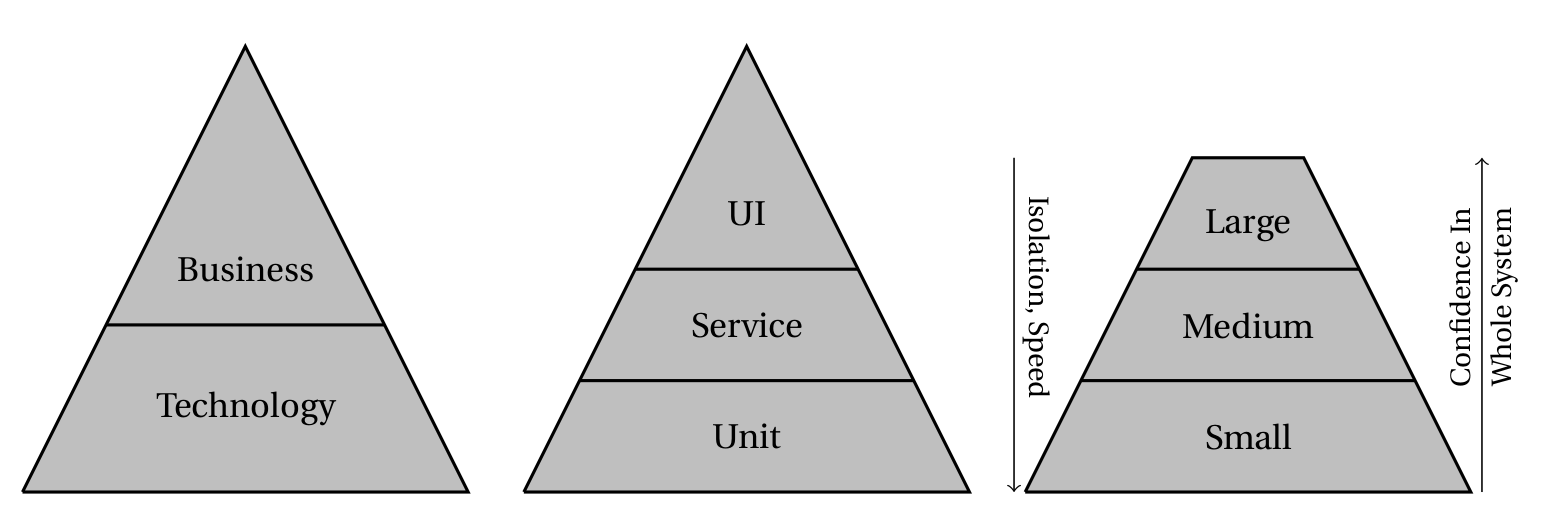
\includegraphics[width=0.9\textwidth]{testing_pyramide}
		\caption{Softwaretestpyramide}
		\label{[softwaretestpyramide]}
	\end{center}
\end{figure}

Die Softwaretestpyramide, die in \ref{[softwaretestpyramide]} visualisiert ist, basiert auf Alister Scott ~\footcite[Vgl.]{website:scott.2011}, Martin Fowler
 ~\footcite[Vgl.]{website:fowler.2012} und Google  ~\footcite[Vgl. Seite 12-14]{Whittaker.2012} (von links nach rechts).


\subsubsection{Integrationstests}
Mit Systemtests wird ein System in seiner Gesamtheit unter Bedingungen getestet, die nah
am realen Betrieb liegen. Ein Systemtest soll zeigen, dass sich das System in den verschiedenen
Nutzungsfällen so verhält, wie man es laut Spezifikation erwartet. Der Gegenpol dazu sind
Unit-Tests, mit denen Code in möglichst kleinen Einheiten isoliert getestet wird. Dabei möchte
man sicherstellen, dass die einzelnen Einheiten jeweils für sich alleine wie erwartet funktionieren.

Integrationstests schließen die Lücke zwischen diesen beiden Testkonzepten, indem sie
auf die Schnittstellen zwischen Komponenten fokussieren und sicherstellen, dass ihr Zusammenspiel
wie erwartet funktioniert. Sie stellen den in der Praxis vielleicht wichtigsten
Baustein im Testkonzept dar, denn Systemtests sind zu groß, um eine hinreichend genaue
Aussage über die Quelle eines Fehlers zu machen. Unit-Tests dagegen sind zu klein, um
eine verwertbare Aussage über das Verhalten der gesamten Anwendung zu machen.

Hinzu kommt, dass Systemtests eine komplexe Test-Umgebung und viele Systemressourcen
zur Ausführung benötigen. Sie sind damit zu langsam und zu teuer, um als Fundament
einer Teststrategie zu dienen. Es gibt Unternehmen, in denen die Ausführung aller
Systemtests mehrere Stunden dauert. Für ein zeitnahes Feedback besonders über
diejenigen Fehler, die im Rahmen der Pflege oder Weiterentwicklung gerade neu eingeführt
wurden, werden Tests in einem kleineren Wirkungsbereich benötigt. Nur diese helfen den
Entwicklern dabei, aufgetretene Fehler unmittelbar den kürzlich vorgenommenen Änderungen
zuzuordnen. Dauert es zu lange, bis das Feedback beim Entwickler eintrifft, ist Testen
im Sinne agiler Software-Entwicklung nicht mehr möglich.

Integrationstests stellen sicher, dass mehrere Code-Einheiten, deren korrektes Verhalten in
Isolation voneinander bereits durch Unit-Tests sichergestellt wurde, wie erwartet zusammenarbeiten.
Testet man dabei von einer System- oder Komponentengrenze bis zu einer anderen solchen Grenze, spricht
man von Edge-to-Edge-Tests.

Aufbauend auf den Ergebnissen der Integrationstests stellt man mit End-to-End-Systemtests in
Form von Akzeptanztests sicher, dass das System sich so verhält, wie es der Auftraggeber erwartet.

Generell gilt, dass jeder Test in einer möglichst minimalen Test-Umgebung ausgeführt werden
sollte. Ein Systemtest beispielsweise benötigt normalerweise eine mit sinnvollen Testdaten
initialisierte Testdatenbank, hat Abhängigkeiten auf externe Systeme etwa für Bonitätsprüfungen,
zur Zahlungsabwicklung oder zum Datentransfer von und in ERP-Systeme wie SAP oder Navision.
In der Realität ist es alles andere als einfach, ein solches Testsystem aufzusetzen, zumal
regelmäßig aktuelle Daten aus dem Produktionssystem in das Testsystem transferiert werden sollten,
da oftmals Tests mit veralteten Daten nicht richtig funktionieren.

Selbst wenn man die Installation eines Testsystems vollständig automatisiert hat, dauert
diese relativ lange. Nach der Ausführung eines Tests hat man dann entweder die Möglichkeit,
ganz im Sinne von Unit-Tests das Testinventar (und damit das gesamte Testsystem)
wieder zu verwerfen und für den nächsten Test neu zu installieren. Selbst wenn man, was
durchaus empfehlenswert ist, zu diesem Zweck mit Schnappschüssen (Snapshots) von virtuellen 
Maschinen arbeitet, so wird die Ausführung der Systemtests insgesamt doch quälend langsam.

Eine andere Möglichkeit ist es, mehrere Tests gegen ein Testinventar auszuführen und
die Veränderungen, die jeder Test am System vornimmt, hinzunehmen. Hierbei verzichtet
man allerdings auf die Testisolation, was zu Wechselwirkungen zwischen Tests führen
kann. Spätestens wenn ein Test fehlschlägt und das System in einem inkonsistenten und
unerwarteten Zustand hinterlässt, ist die Wahrscheinlichkeit hoch, dass – gewissermaßen
als Folgefehler – weitere nachfolgende Tests ebenfalls fehlschlagen. Das macht es nicht
gerade einfach, die ursprüngliche Fehlerquelle zu finden.

Man sieht, dass es sehr sinnvoll ist, Tests in einer minimalen Umgebung auszuführen.

\subsubsection{GUI-Tests}
Unter \nomenclature{GUI}{Graphical user interface}GUI-Tests versteht man die automatische Überprüfung der Benutzeroberfläche eines Anwenders.
Dies sorgt dafür das alle Schaltflächen in der GUI die gewohnten Funktionen ausführen und nicht mit falschen Endpunkten verknüpft sind.

\subsubsection{Regressionstests}
In der Entwicklung sollte nach jeder Änderung ein Regressionstest ausgeführt werden. Bei Regressionstest
müssen Sie darauf achten, dass 1) Sie immer die gleichen Tests ausführen, wenn Sie einen
bestimmen Code-Abschnitt testen und 2) das betreffende Tests die Akzeptanzkriterien der jeweiligen
Anforderung abgleicht. Wenn nun später aber Jenkins in den Testprozess integriert würde, könnte
man sich diese Arbeit sparen. Mit Jenkins würde es dann möglich sein, die Regressionstest regelmäßig
auszuführen, etwas nach jeder Codeänderung oder einmal pro Nacht (Nightly Build). Falls Probleme auftreten sollten,
würde das Team per Email, HipChat oder ähnlichen Kommunikationswege informiert.

\subsubsection{Mutation-Testing}\label{mutation-testing}

Mutation-Testing (auch Mutation Analyse oder Programm Mutation genannt) wird verwendet um neue Software-Tests zu erstellen und die Qualität der vorhandenen Tests zu evaluieren. Die Durchführung von Mutation-Testing ist in der Theorie ziemlich einfach, das vorhandene, zu testende, Programm wird an wenigen Stellen verändert. Jede so neu entstandene Version dieses Programms nennt man Mutant. Jeder erstellte Mutant wird mit den vorhandenen Tests überprüft um zu verifizieren, dass sich die Test-Suite anders verhält und somit die Änderung an dem Programm bemerkt. Tritt dieser Fall ein, spricht man vom \dq{}killing the mutant\dq{}. Die existierende Test-Suite wird anhand der prozentualen entdecken von Mutanten bewertet. Desto höher dieser Wert ist, umso genauer sind die automatisierten Tests in der Überprüfung und Validierung der Software. 

Um diesen Richtwert zu erhöhen, können neue Tests erstellt werden die genau so eine auftretende Mutation überprüfen. Mutationen basieren auf wohldefinierten Veränderungen wie zum Beispiel typische Programmierfehler (Verwendung des falschen Operator oder Variablennamen). Zweck dieser ganzen Veränderungen ist es dem Softwareentwickler zu unterstützen, bessere und effektivere Tests zu schreiben. Ein weiterer Aspekt ist die Identifizierung von schwächen in den verwendeten Testdaten oder selten genutzten Funktionen. Dies sind alles unterstützende Faktoren die dem Softwareentwickler helfen können, um bessere Software-Tests zu entwickeln.

Mutation-Testing gehört zu der Gruppe der White-Box Tests.

\subsection{Testgetriebene Entwicklung}
Wenn eine neue Funktionalität in einem Programm implementiert bzw. eine Funktionalität angepasst und erweitert werden soll, wie stellt man sicher, dass es im Nachhinein
zu keinerlei Problemen kommt? Die Funktionalität per Hand zu testen ist aus mehreren Gründen nicht vorteilhaft.

Die testgetriebene Entwicklung versucht dieses Problem zu beheben. Um dieses Ziel zu erreichen, wird zu Erst mit einem Test die Funktionalität spezifiziert. Nach der
Fertigstellung des Tests wird der Programmcode entwickelt. Das führt dazu, dass nun die komplette Funktionalität überprüft werden kann. Wenn unerwünschte Seiteneffekte 
entstehen, die auf Grund einer Codeänderung an einer anderen Stelle auftreten, können sie nun durch die Tests herausgefunden und dadurch
behoben werden.

\subsection{Verhaltensgetriebene Entwicklung}
BDD wurde ursprünglich 2003 von Dan North als Weiterentwicklung von TDD bekannt gemacht. 6

Dan North führte dabei syntaktische Konventionen für Unit-Tests ein. Als „Unit-Tests“ bezeichnet man Überprüfungen ob Komponenten wie gewünscht funktionieren. Er
entwickelte „JBehave“ als Ersatz für „JUnit“, das alle verwandten Wörter von „Test“ mit dem Wort „Verhalten“ ersetzt hat. „JUnit“ ist ein Framework zum Testen von Java-
Programmen welches von „JBehave“ durch veränderte Namenskonventionen abgelöst wurde.

Wieso führte Dan North eine Vokabular Umstellung durch? Edward Sapir und Benjamin Whorf bildeten eine Hypothese die aussagt, dass die Sprache, die wir nutzen, unser 
Denken beeinflusst 7 . Wollen wir unsere Denkweise verändern, hilft es demzufolge nach, die Sprache zu verändern.

Die Testgetriebene Entwicklung führte dazu, dass viele Entwickler den Entwicklungszyklus nicht optimal verwendet haben. Deswegen kam Dan North auf die Idee, durch
Namenskonventionen das Verhalten in den Mittelpunkt zu rücken. Die Basis von BDD sind flexible Methoden, die darauf abzielen, Teams mit wenig Erfahrung in agiler 
Softwareentwicklung, den Einstieg zugänglicher und effizienter zu gestalten.


